\documentclass{article}
\usepackage{graphicx}
\usepackage{subcaption}
\usepackage{amsmath}
\usepackage{amssymb}
\usepackage{amsthm}
\usepackage[backend=biber,style=numeric,sorting=none]{biblatex}
\addbibresource{references (5).bib}


\title{MCMC Algorithms}
\author{Srotoshi Ghosh}
\date{November 2024}

\begin{document}

\maketitle

\section{Introduction}
 Markov Chain methods use a process which draws samples in same proportions as the target distribution, implying that the number of samples drawn will be greater from where the value of the target distribution PDF is higher. The key principle of MCMC is setting up a random walk over the parameter space preferentially exploring regions of high probability densities. Such a specific random walk is performed using a Markov Chain. 

\section{Definition}
\begin{itemize}
    \item A Markov chain is a stochastic process characterized by the principle that the future state $\theta_{t+1}$ depends only on the present state $\theta_t$, through a transition probability $Q(\theta_{t+1}|\theta_t)$, and not on the sequence of events that preceded it \cite{bailer2017practical,10.1119/5.0122488}.This is the property of memorylessness.
    \item The set of samples selected from a proposal distribution to represent the target distribution through this process is known as a Markov chain.
    \item In other words, a Markov chain consists of a set of states and transition probabilities between these states, which define the likelihood of moving from one state to another.
    \item A Markov chain must asymptotically reach a stationary or equilibrium distribution in which it remains in forever, after reaching it, and this stationary distribution must be equal to the target distribution of the sampling process.
    \item This is possible only if the "detailed balance" condition is achieved. The condition of "detailed balance" implies that Markov chains are reversible.
    \item  In other words, it means that it is equally probable for the chain to transform from a state $\theta_a$ to a state $\theta_b$ as the probability of transforming from state $\theta_b$ to $\theta_a$. This condition signfies some form of an equilibrium, ensuring that the system does not favour any particular direction of transition and that the samples collected represent the target distribution accurately. 
\end{itemize}
\begin{figure}
    \centering
    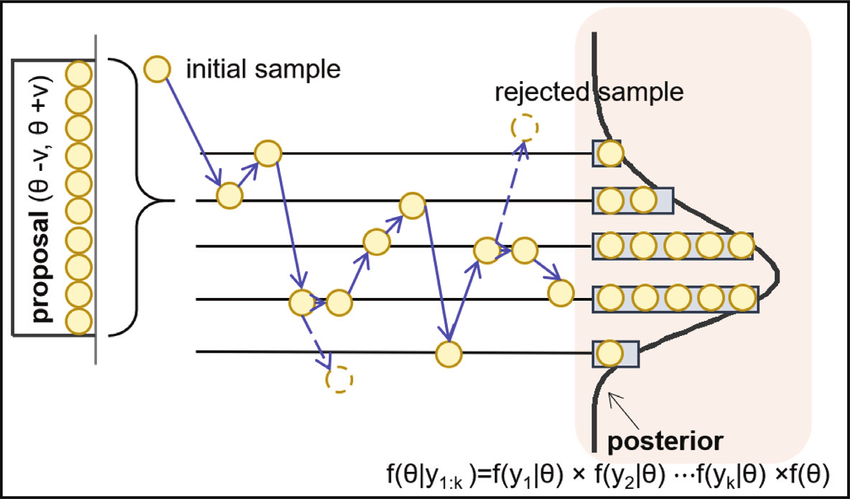
\includegraphics[width=0.5\linewidth]{mcmc.png}
    \caption{This image demonstrates the process of Markov Chain Monte Carlo sampling from a proposal distribution such that the Markov Chains converge to the desired target distribution}
    \label{fig:mcmcdemo}
\end{figure}

\section{Proposal and Target Distributions}

\begin{enumerate}
    \item Proposal Distribution :
    The proposal distribution is a probability distribution used to suggest new states or points to sample from, based on the current state in the Markov chain. It defines how new candidate points are proposed for the next iteration. The role of the proposal distribution is to guide the exploration of the parameter space and determine which points are considered as candidates in each step.

    \item Target Distribution :
    The target distribution is the distribution that the samples drawn from proposal distribution must converge to. The goal of MCMC is to produce a sequence of samples that approximate this distribution.
\end{enumerate}

\section{Metropolis-Hastings Sampling Algorithm}
The Metropolis-Hastings algorithm is widely used for obtaining a sequence of random samples from a probability distribution for which direct sampling is difficult. This algorithm generates a Markov chain that has the desired distribution or the target distribution as its equilibrium distribution \cite{bailer2017practical,bolstad2016introduction}. It is especially useful in Bayesian statistics where one needs to draw samples from complex, high-dimensional distributions.

The Markov Chain is initialized with some specific value, and proceeds iteratively. A random sample $s$ is drawn from the proposal distribution $Q(s|\theta_t)$ where $\theta_t$ is the given value of parameter, and $s$ is utilized to determine the best value of the parameter in the next iteration, denoted as $\theta_{t+1}$. We determine whether the sample is accepted or not through the calculation of the Metropolis ratio or acceptance probability. The acceptance probability $\alpha$ is expressed as:
\begin{equation}
\alpha = min\left( 1, \quad \frac{g(s) \quad Q(\theta_t|s)}{g(\theta_t) \quad Q(s|\theta_t)} \right) \label{eq:mhalg}
\end{equation}
Here, $g(\theta_t)$ is the target distribution. We generate a random number $u$ from the uniform distribution $U(0,1)$. If $u \leq \alpha$, then, $\theta_{t+1}$ is set as the sample $s$ and our proposal candidate is accepted. Otherwise, the sample is rejected and $\theta_{t+1}$ is set as $\theta_t$. The iterative procedure is repeated for a large number of steps, allowing the samples to converge to the target distribution. 

The decision rule for Metropolis-Hastings algorithm ensures that the random walk over the sample space goes mostly uphill, towards higher probability densities, but also allows downhill moves. This ensures the exploration of the entire distribution with preference over regions of higher probability densities. 

The acceptance probability $\alpha$ ensures that the Markov chain satisfies the detailed balance condition, which is necessary for the chain to have the correct stationary distribution. This probability corrects for any biases introduced by the proposal distribution. Further, the resulting chains are inspected for the presence of right properties as predicted by the target distribution. To ensure that the chains have reached steady state, sampling is rerun several times and convergence to same region of parameter space despite different initial starting points are checked.

As the number of iterations increases, the distribution of the states visited by the chain approaches the target distribution. Initially, the chain may take some time to "burn-in" or converge to the stationary distribution, after which the samples can be used for estimation. The initial samples generated before the chain reaches its stationary distribution are often discarded. This period is known as the burn-in period.

The choice of the proposal distribution is crucial for the efficiency of the algorithm. It may be symmetric, like a Gaussian centered at the current state $\theta_t$ or asymmetric. If the proposal is symmetric, the factor  A good proposal distribution balances exploration and exploitation, ensuring the chain moves through the state space efficiently. A poor choice can lead to high rejection rates and slow mixing, meaning the chain takes longer to explore the state space.

\section{Gibbs Sampling}

Gibbs sampling is a special MCMC method used to generate a sequence of samples from a multivariate probability distribution or for a multi-parameter target distribution \cite{bolstad2016introduction}. It is particularly useful when direct sampling from the joint distribution is difficult, but sampling from the conditional distributions of parameters is feasible.

Gibbs sampling cycles through each parameter, sampling from its conditional distribution given the latest values of the other parameters and the data, ensuring convergence to the join target distribution. This method simplifies the sampling process by using the hierarchical structure to derive the required conditional distributions.

Though it can handle multiple parameters, its efficiency often decreases as the increase in the number of parameters lowers the acceptance rates. The Gibbs sampling is a special case of the block-wise Metropolis-Hastings algorithm, specifically when the true conditional density of a parameter block given the other parameters can be derived. It has its domain own domain of applicability in spite of drawbacks. 

Instead of proposing a random sample density at each point, we consider the true conditional density for every parameter given all of the others as the candidate or sample to be accepted or rejected. Assuming $\theta_{-j}$ is the set of all the parameters excluding the $j^{th}$, we can write:
\begin{equation}
Q(\theta_j,\theta^{'}_j|\theta_{-j}) = g(\theta_j|\theta_{-j}) \nonumber
\end{equation}
Here, $Q$ represents the proposal distribution and $g$ represents the target distribution. The acceptance probability for $\theta_j$ at the $n^th$ iteration is: 
\begin{equation}
\alpha (\theta^{(n-1)}_j,\theta^{'}_j|\theta^{(n)}_{-j}) = min \left( 1, \quad \frac{g(\theta^{'}_j|\theta_{-j}) \quad Q(\theta^{'}_j,\theta_j|\theta_{-j})}{g(\theta_j|\theta_{-j}) \quad Q(\theta_j,\theta_j|\theta_{-j})} \right) \label{eq:gibbssamp}
\end{equation}
Here, the acceptance probability always comes out to be 1 due to our choice of proposal distribution as the true conditional distribution of parameters. Hence, the candidate is accepted at each state. The accepted candidate is used to generate the next candidate for another parameter, and that too is accepted. This is how the algorithm proceeds iteratively. 

Gibbs sampling relies on the ability to sample from the conditional distributions. Each variable is changed sequentially in one complete iterative cycle by updating each variable based on the latest values of the other variables. This ensures that the Markov chain generated by Gibbs sampling converges to the target distribution, allowing for estimation of its properties. However, an initial burn-in period is often required to allow the chain to converge to the stationary distribution. Samples generated during this period are typically discarded.

\section{Summary of Algorithms}
\begin{minipage}[t]{0.55\textwidth}
        \centering
        \textbf{Metropolis-Hastings Algorithm } \\
        \begin{itemize} 
            \item  $s$ is a random sample drawn from proposal distribution $Q(s|\theta_t)$ 
            \item calculation of the Metropolis ratio or acceptance probability:
            \begin{equation}
                \alpha = min\left( 1, \quad \frac{g(s) \quad Q(\theta_t|s)}{g(\theta_t) \quad Q(s|\theta_t)} \right) \nonumber
            \end{equation}
            $g(\theta_t)$ is the target distribution. 
            \item generation of $u$ from the uniform distribution $U(0,1)$
            \item if $u \leq \alpha$, then, $\theta_{t+1}=s$  or else $\theta_{t+1}=\theta_t$. 
        \end{itemize}
    \end{minipage}%
    \begin{minipage}[t]{0.55\textwidth}
        \centering
        \textbf{Gibbs Sampling Algorithm} \\
        \begin{itemize}
            \item $\theta_{-j}$ is the set of all the parameters excluding the $j^{th}$:
            \begin{equation}
                 Q(\theta_j,\theta^{'}_j|\theta_{-j}) = g(\theta_j|\theta_{-j}) \nonumber
            \end{equation}
            $Q$ : proposal distribution, $g$ : target distribution. 
            \item The acceptance probability for $\theta_j$ at the $n^{th}$ iteration is: 
            \begin{equation}
                \alpha = min \left( 1, \frac{g(\theta^{'}_j|\theta_{-j}) Q(\theta^{'}_j,\theta_j|\theta_{-j})}{g(\theta_j|\theta_{-j}) Q(\theta_j,\theta_j|\theta_{-j})} \right) \nonumber 
            \end{equation} 
            \item The sample for each parameter chosen from conditional distribution of parameter, and utilized to generate the other parameters at each state.
            
        \end{itemize}
    \end{minipage}

\printbibliography

\end{document}